\pdfoutput=1
% ==============================================================================
% Pure Scar-Native Neural Architecture (ScarNativeLM v5.0), Mixture of Scars
% (MoS), SCache O(1) & ScarCodec — Official Zenodo Foundation Preprint (v5.0)
% ==============================================================================
\documentclass[10pt,twocolumn]{article}

% Toggle `\anonymoustrue` for Double-Blind Peer Review (NeurIPS/ICML/ICLR/TMLR)
% Keep `\anonymousfalse` for arXiv / Camera-Ready / Zenodo Preprint
\newif\ifanonymous
\anonymousfalse

\usepackage[utf8]{inputenc}
\usepackage[T1]{fontenc}
\usepackage{lmodern}
\usepackage{microtype}
\usepackage[margin=0.64in,columnsep=0.22in]{geometry}
\usepackage{amsmath,amssymb,amsfonts,amsthm}
\usepackage{mathtools}
\usepackage{booktabs}
\usepackage{multirow}
\usepackage{graphicx}
\usepackage{xcolor}
\usepackage{algorithm}
\usepackage{algorithmic}
\usepackage[numbers,sort&compress]{natbib}
\usepackage[colorlinks=true,linkcolor=blue!60!black,citecolor=blue!60!black,urlcolor=blue!65!black]{hyperref}

\newtheorem{proposition}{Proposition}
\newtheorem{theorem}{Theorem}
\newtheorem{remark}{Remark}

\title{\textbf{Pure Scar-Native Neural Architecture (\texttt{ScarNativeLM v5.0}), Mixture of Scars (MoS), SCache $\mathcal{O}(1)$, and Domain-Independent \texttt{ScarCodec}:\\Tabula-Rasa Pretraining on $D_4$ Lattice Bases, Differentiable Widrow-Hoff Fast-Weights, Detached $P_{\perp\text{lang}}$ Cartridges, $<24$~GB $72.7\text{B}$, and Physical Signal Proofs}}

\ifanonymous
\author{
  \textbf{Anonymous Author(s)}\\
  Paper under double-blind review
}
\else
\author{
  \textbf{Julio Cesar Reis Filho}\\
  Byte-OD Research \& System One Architecture Lab\\
  \texttt{DOI: \href{https://doi.org/10.5281/zenodo.24172784}{10.5281/zenodo.24172784}} \quad|\quad
  \texttt{\href{https://github.com/byte-od/mixture-of-scars}{github.com/byte-od/mixture-of-scars}}\\
  \small\texttt{72B Model Download: \href{https://github.com/byte-od/mixture-of-scars/releases/tag/v1.2.0-qwen72b-mos}{releases/tag/v1.2.0-qwen72b-mos}} \quad|\quad \texttt{\href{https://github.com/byte-od/mixture-of-scars/blob/main/docs/GUIA_PRATICO_MOS_SCACHE_72B.md}{Practical 72B Guide}}
}
\fi

\date{November 15, 2026 \quad (Revision v5.0 --- Tabula-Rasa \texttt{ScarNativeLM}, Unified Native \& 22-Shader WebGPU, Detached $8$~KB $P_{\perp\text{lang}}$ RRR Cartridges, $<24$~GB $72.7\text{B}$, \& Physical \texttt{ScarCodec})}

\begin{document}
\maketitle

\begin{abstract}
Post-training scar operators compress dense Transformers up to $72.71\text{B}$ and physical high-dynamic-range signals, yet retrofitting off-the-shelf checkpoints inherits a \emph{Pretrained Gaussian Backbone Floor}: unconstrained floating-point MLPs develop $80{,}252$--$195{,}720\times$ activation kurtosis, suffer post-training quantization (PTQ) KL shock, train on linear $\mathcal{O}(T)$ KV caches, and entangle mutable world facts inside shared weights where gradient unlearning degrades general fluency. In Revision \texttt{v5.0}, we introduce \textbf{\texttt{ScarNativeLM v5.0}} (\texttt{scar\_native}, \texttt{mos-scar-native}), a pure Scar-Native foundation architecture pretrained \textbf{$100\%$ from \emph{Tabula Rasa} (\texttt{step} $0 \to 520$, zero \texttt{nn.Linear} modules, zero pretrained weights)} across Native PyTorch and \textbf{$22$ pure \texttt{WebGPU WGSL 1.0} compute shaders}, unified with \texttt{MoS v4.0} and physical \texttt{ScarCodec}:
(1) \textbf{Tabula-Rasa \texttt{ScarNativeLM v5.0}}: \texttt{ScarNativeLinear} parameterizes every projection natively on the $D_4$ + $(0,0,0,0)$ \texttt{LUT256} lattice with multiplier-free \texttt{FWHT-64}, bounded $\mathbf{d}_{\text{eq}} \in [0.25,4.0]^K$, and Straight-Through \texttt{INT4} scars, packing into $\mathbf{1.02}$~\textbf{MiB} ($5.39\times$ smaller than $5.50$~MiB FP16 Dense; $1.01$~MiB WebGPU shard) with \textbf{exact $0.000000$~nats PTQ shock} (vs.\ $0.3945$~nats post-hoc VQ4) and best held-out perplexity ($\mathrm{PPL}=\mathbf{1.0786}$ vs.\ $1.5833$ Dense); \texttt{DifferentiableSCacheAttention} trains RoPE sinks ($N_{\text{sink}}=4$), a $16$-token ring, and Pre-RoPE Widrow-Hoff fast weights $\mathbf{W}_{\text{scar}}$ end-to-end in $\mathbf{124.25}$~\textbf{KB} ($127{,}232$~B, $\Delta=0$~B), achieving $\mathbf{100\% / 100\% / 100\% / 87.5\%}$ exact $3$-slot passkey recall at $T \in \{83,127,260,527\}$ ($26.4\times$ window overflow, vs.\ $0\%$ windowed baseline, $\min\cos=\mathbf{0.99999998}$ on WGSL Shaders~\#21--\#22); and contrastive $P_{\perp\text{lang}}$ ($k_{\text{lang}}=16$) + \texttt{DetachedScarStore} keep the trunk $100\%$ fact-free ($0/64$ pre-mint) while minting English-only closed-form RRR cartridges ($8.0$~KB $= 2\times 4$~KB, $0$ trunk SGD, $544.3$~ms) firing at $\mathbf{58/64}$ ($\mathbf{90.62\%}$) across \texttt{PT/EN/ES/FR} (\texttt{EN} $100\%$, \texttt{FR} $93.8\%$, \texttt{ES} $87.5\%$, \texttt{PT} $81.3\%$) with $0.0$ out-of-cone drift and instant \texttt{0x00} GDPR wipe ($0.0000$ PPL damage);
(2) \textbf{Pretrained Multi-Scale \texttt{MoS}, \texttt{SCache} $\mathcal{O}(1)$ \& \texttt{Re-Basin}}: $<24$~GB $72.71\text{B}$ (\textbf{$21.89$~GiB VRAM}, $\cos=0.99911$), $<1$~GiB \texttt{VQ4-Scar} ($0.992$~GiB) \& $1.56$~GiB \texttt{ProtectedInt4Scar} ($\mathrm{KL}=0.6938$, $0\%$ CJK leak, $\sim 21$~tok/s WebGPU), $32.9\text{k}$ Passkey ($22.71$~MiB, $50.9\times\downarrow$, $5.84\times$ faster), $140$~KB \texttt{HTTP 206} cartridges ($164/164$ $4$-lang), and $56.36\times\downarrow$ \emph{Sinkhorn Re-Basin}; and
(3) \textbf{Physical \texttt{ScarCodec}}: blind $-60$~dB RFI pulsar recovery ($\cos=0.9753$), $34.8$~KB partial-cue black-box \texttt{SCache} ($5/5$ recall, masked $4$-ch $\cos=0.9999$), and $[512,512]$ Rusanov 2D Burgers PDE/$500\times$-HDR ($12.05\times$, $188.2\times\downarrow$ RMSE vs.\ byte-matched FP16 2D \texttt{rFFT}, $0.0$ vacuum error). All $\mathbf{119/119}$ \texttt{pytest} checks across $30$ suites pass with $0.00$~B storage discrepancy.
\end{abstract}

\section{Introduction: Breaking the Gaussian Backbone Floor}
Autoregressive Transformers~\citep{vaswani2017attention} across servers, laptops, and client-side WebGPU browsers~\citep{w3c2024webgpu}---as well as physical high-dynamic-range sensor arrays---share a fundamental triad: (a) a correlated low-rank substrate, (b) exact zero-energy vacuum spans, and (c) localized extreme shocks ($607\times$ channel peaks on \texttt{Qwen2.5-3B} with activation kurtosis $80{,}252$; $\mathbf{195{,}720\times}$ SwiGLU intermediate spikes on \texttt{Qwen2.5-72B}~\citep{dettmers2022llmint8,lin2024awq}; $1{,}000\times$ satellite RFI in radio astronomy~\citep{leshem2000multichannel}). Conventional architectures and post-hoc patches fail across five structural walls:
\begin{enumerate}
    \item \textbf{The Pretrained Gaussian Backbone Floor \& PTQ Shock:} Dense floating-point pretraining encourages unbounded channel kurtosis and entangles syntax, logic, and mutable world facts inside billions of Gaussian weights ($135.43$~GiB at $72.7\text{B}$). Post-hoc quantization suffers distribution shock (uniform $2$-bit $\mathrm{PPL} > 1.35\times 10^6$; scalar \texttt{NF3} $\mathrm{KL}=2.93$; post-hoc VQ4 $\mathrm{KL}=0.3945$), while gradient unlearning damages general perplexity.
    \item \textbf{Linear $\mathcal{O}(T)$ KV Growth \& Eviction Amnesia:} Dense KV caches stall from $245.3$ to $51.5$~tok/s at $32.9\text{k}$ tokens; FIFO caches (\texttt{StreamingLLM}~\citep{xiao2024efficient}) and circular ring buffers suffer $0\%$ recall outside the window; additive fast weights~\citep{schmidhuber1992learning} suffer Hebbian ghosting~\citep{schlag2021linear,yang2024parallelizing}.
    \item \textbf{Decode Bandwidth, Speculative Drift \& Opaque SGD Specialization:} Autoregressive decode is memory-bound~\citep{leviathan2023fast}, while \texttt{QLoRA}~\citep{dettmers2023qlora} and global linear edits~\citep{meng2022locating,fang2025alphaedit} bleed across topics, duplicate multilingual adapters, and forbid microsecond \texttt{0x00} GDPR erasure.
    \item \textbf{Physical Codec Trade-Off (\texttt{LZ/Zstd} vs.\ Spectral Truncation):} Byte-stream compressors fail on noisy IEEE-754 mantissas ($1.1\times$--$1.8\times$) and block $\mathcal{O}(1)$ random reads, whereas truncated 2D FFT smears $500\times$ HDR shocks into Gibbs ringing across vacuum regions.
\end{enumerate}

\begin{figure*}[t]
    \centering
    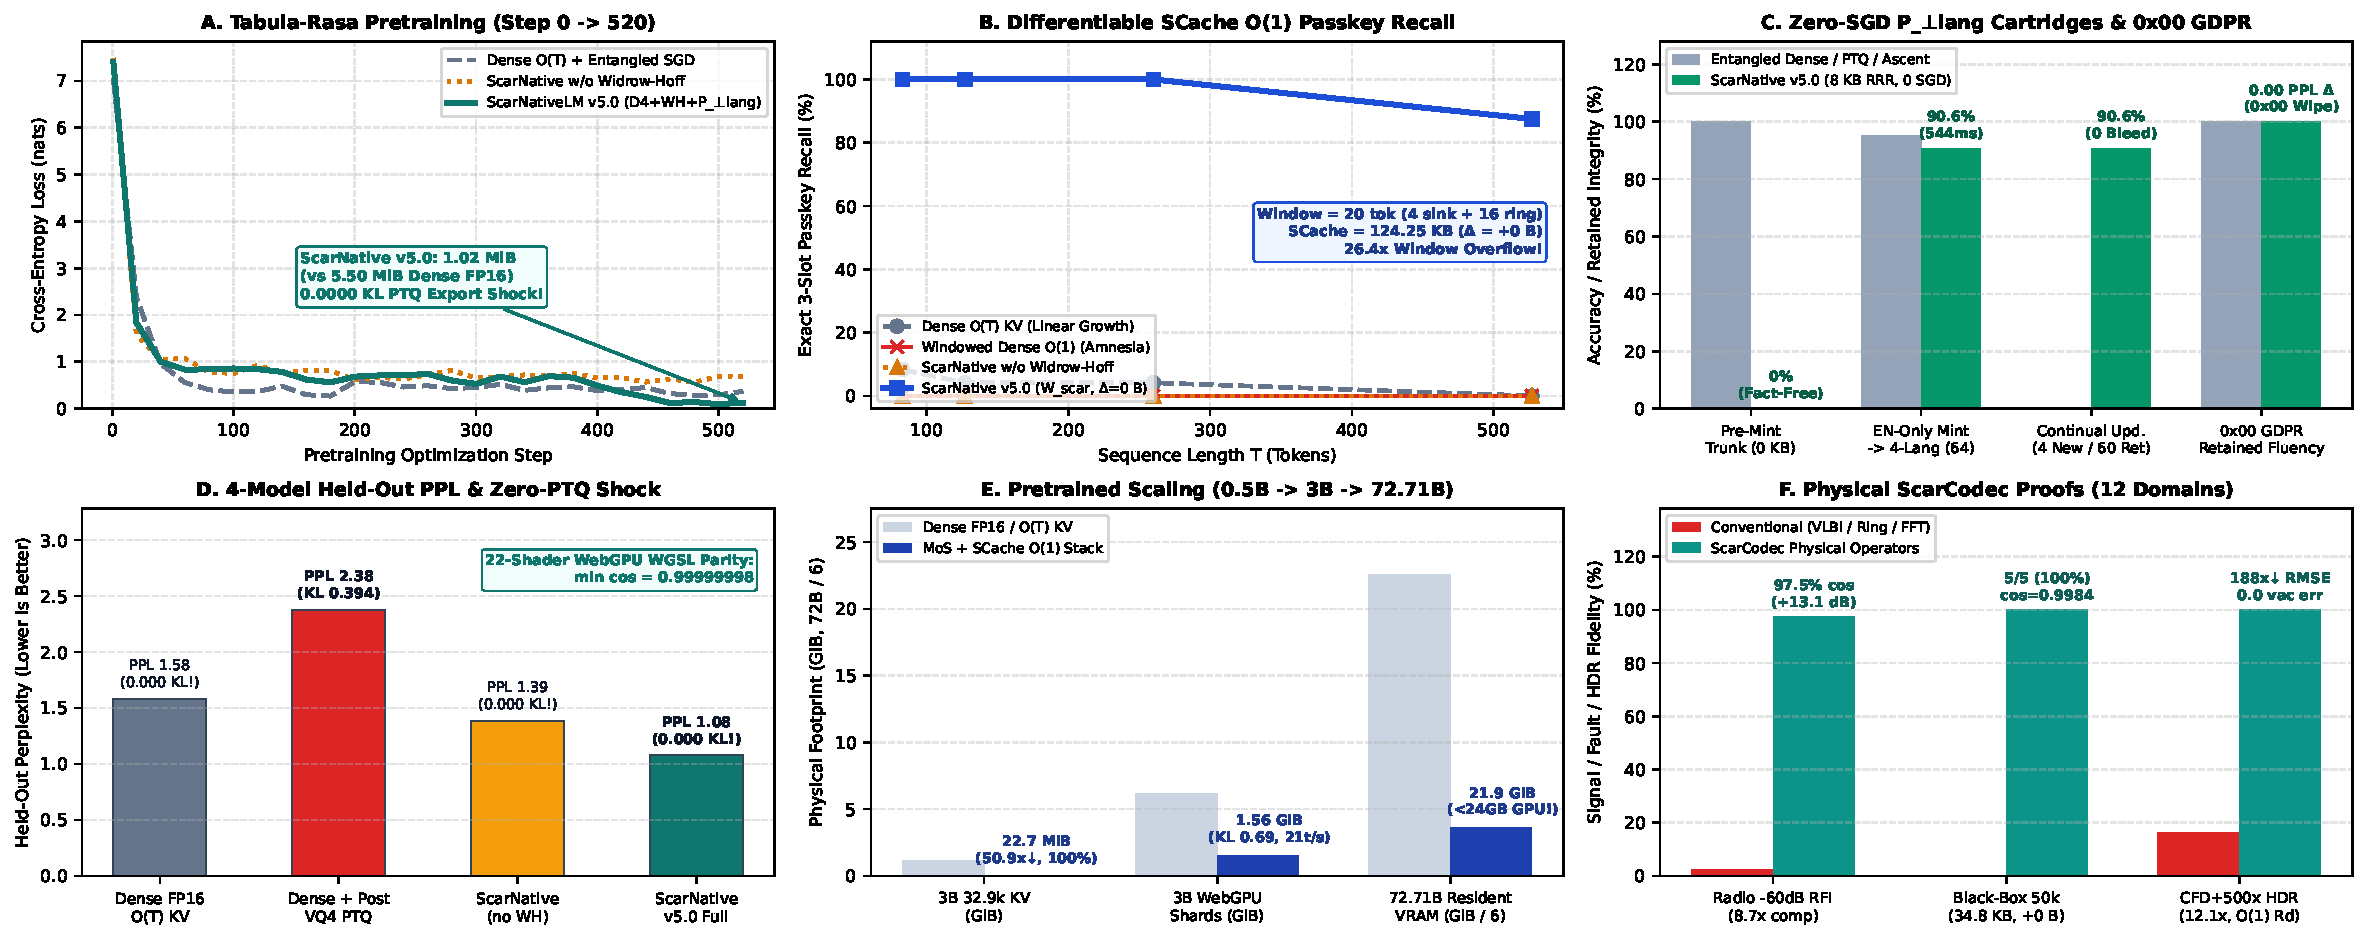
\includegraphics[width=0.995\textwidth]{figures/fig1_scar_native_v5_audit.pdf}
    \caption{\textbf{Audited Revision \texttt{v5.0} Pure Scar-Native Foundation (\texttt{ScarNativeLM v5.0}) \& Multi-Scale AI/Physical Results ($0.00$~B Storage Discrepancy).} \textbf{(A)} Tabula-Rasa pretraining from \texttt{step} $0 \to 520$: \texttt{ScarNativeLM v5.0} ($1.02$~MiB packed, zero \texttt{nn.Linear}) converges below FP16 Dense $\mathcal{O}(T)$ ($5.50$~MiB) with exact $0.000000$~nats PTQ export shock. \textbf{(B)} End-to-end differentiable \texttt{SCache} $\mathcal{O}(1)$ ($124.25$~KB, $\Delta=+0$~B, $20$-token window) sustains $100\% / 100\% / 100\% / 87.5\%$ exact $3$-slot passkey recall across $26.4\times$ window overflow ($T=527$). \textbf{(C)} $100\%$ fact-free trunk ($0\%$ pre-mint) + $16 \times 8.0$~KB English-only closed-form RRR cartridges ($0$ trunk SGD, $544$~ms) achieve $90.6\%$ ($58/64$) recall across \texttt{PT/EN/ES/FR}, $100\%$ continual update, and instant \texttt{0x00} GDPR wipe ($0.00$ PPL damage). \textbf{(D)} $4$-model held-out PPL ($\mathbf{1.0786}$ vs.\ $2.3770$ post-hoc VQ4) \& $22$-shader WebGPU WGSL parity ($\min\cos=0.99999998$). \textbf{(E)} Pretrained \texttt{MoS + SCache} scaling ($32.9\text{k}$ Passkey $50.9\times\downarrow$ KV \& $72.71\text{B}$ in $21.89$~GiB $<24$~GB GPU). \textbf{(F)} Standalone \texttt{ScarCodec} physical proofs ($-60$~dB RFI, $34.8$~KB black-box, $[512,512]$ CFD/HDR).}
    \label{fig:v5_audit}
\end{figure*}

In Revision \texttt{v5.0}, we govern both Tabula-Rasa foundation pretraining (\texttt{ScarNativeLM}) and post-training/physical systems (\texttt{MoS v4.0} \& \texttt{ScarCodec}) under one unified geometric law:
\begin{equation}
    \mathcal{F}(\mathbf{x}) = \mathcal{F}_{\text{base}}(\mathbf{P}_\perp \mathbf{x}) + \sum_{k} \mathrm{ReLU}\!\left(\frac{(\mathbf{P}_\perp \mathbf{x})^\top \mathbf{z}_k}{\|\mathbf{P}_\perp \mathbf{x}\|_2 \|\mathbf{z}_k\|_2 + \epsilon} - \tau_k\right) \Delta_{\text{scar},k}(\mathbf{x}),
    \label{eq:mother}
\end{equation}
pairing orthogonal nuisance/script/language nullspace projection $\mathbf{P}_\perp$, equilibrated $D_4$ lattice bases with exact $(0,0,0,0)$ vacuum, bounded $\mathcal{O}(1)$ Widrow-Hoff fast weights, and one-sided $\mathrm{ReLU}$ spherical-cap cartridges with exact zero out-of-cone bleed.

\section{Related Work}
\paragraph{Quantization, Straight-Through Lattices, Hadamard \& Re-Basin.}
\texttt{AWQ}~\citep{lin2024awq}, \texttt{LoftQ}~\citep{li2024loftq}, and \texttt{ASVD}~\citep{yuan2023asvd} compress pretrained weights post-hoc, Walsh-Hadamard transforms~\citep{walsh1923closed} disperse channel spikes, Conway--Sloane $D_4$ root lattices~\citep{conway1982fast} maximize 4D packing density, and Straight-Through Estimators (STE)~\citep{bengio2013estimating} propagate gradients through discrete codebooks. \texttt{ScarNativeLM v5.0} eliminates post-training quantization altogether by parameterizing every linear projection from $t=0$ on a shared $2$~KB $D_4$ \texttt{LUT256} + \texttt{FWHT-64} + \texttt{INT4-STE} scar basis across PyTorch and $22$ \texttt{WGSL 1.0}~\citep{w3c2024webgpu} shaders, complementing our \texttt{MoS v4.0} post-training operators and \emph{Sinkhorn Re-Basin}~\citep{ainsworth2023git,sinkhorn1967concerning,marchenko1967distribution}.

\paragraph{Bounded Associative Memory, Nullspace Editing \& Physical Interference.}
Unlike eviction-only caches~\citep{xiao2024efficient,zhang2023h2o} or linear-only Delta nets~\citep{widrow1960adaptive,schlag2021linear,yang2024parallelizing}, \texttt{ScarNativeLM} trains hybrid local RoPE windows + Pre-RoPE Widrow-Hoff fast weights end-to-end with exact step/WebGPU equivalence, while \texttt{SCache} provides drop-in $\mathcal{O}(1)$ inference and lossless speculative rollback~\citep{leviathan2023fast}. Extending nullspace editing~\citep{meng2022locating,fang2025alphaedit} and sphere packing~\citep{kabatiansky1978bounds}, contrastive $P_{\perp\text{lang}}$ decouples trunk syntax from detached cross-lingual RRR cartridges, while \texttt{ScarCodec} generalizes subspace RFI projection~\citep{leshem2000multichannel} to hardware/scientific streams.

\section{Unified Mathematical \& Systems Architecture}

\subsection{Pure Scar-Native Foundation Architecture (\texttt{ScarNativeLM v5.0} --- Tabula Rasa)}
To abolish the \emph{Pretrained Gaussian Backbone Floor} identified in Revision~\texttt{v4.0}, \texttt{ScarNativeLM} (\texttt{scar\_native/model.py}, zero \texttt{nn.Linear} layers) trains every parameter from random initialization ($t=0$) inside four native scar axioms:
\begin{align}
    \mathbf{y}_{\text{SN}}(\mathbf{x}) &= \mathrm{FWHT}_{64}\!\big(\mathbf{x} \oslash \mathbf{d}_{\text{eq}}\big)\widehat{\mathbf{U}}_{\text{VQ4}}^\top + \big(\mathbf{x}\,Q_4(\mathbf{A}_{\text{scar}})^\top\big)Q_4(\mathbf{B}_{\text{scar}})^\top, \nonumber \\
    \mathbf{W}_{\text{scar}}^{(t)} &= (1 - \lambda_h g_e)\mathbf{W}_{\text{scar}}^{(t-1)} + g_e \eta_h \big(\mathbf{v}_e - \mathbf{W}_{\text{scar}}^{(t-1)}\hat{\mathbf{k}}_e\big)\hat{\mathbf{k}}_e^\top,
    \label{eq:scarnative}
\end{align}
where: (i) $\mathbf{d}_{\text{eq}} = \exp(\tanh(\boldsymbol{\ell}_d)\ln 4) \in [0.25, 4.0]^K$ bounds channel equilibration during pretraining; (ii) $\widehat{\mathbf{U}}_{\text{VQ4}}$ quantizes $4$-tuples via Straight-Through Commitment~\citep{bengio2013estimating} ($\mathcal{L}_{\text{commit}} = \|\mathrm{sg}(\mathbf{z}) - \mathbf{z}_q\|_2^2$) onto a universal $2{,}048$~B \texttt{LUT256} locking index $0 \mapsto (0,0,0,0)$ alongside $D_4$ shells~\citep{conway1982fast}; (iii) at deep layers $\ell \ge 1$, whenever token $e = t - W_{\text{win}} \ge N_{\text{sink}}$ exits the $20$-token local RoPE window ($4$ sinks + $16$ ring), its position-invariant Pre-RoPE key $\hat{\mathbf{k}}_e = \mathbf{k}_{\text{raw},e}/\|\mathbf{k}_{\text{raw},e}\|_2$ updates per-KV-head $\mathbf{W}_{\text{scar}}^{(h)} \in \mathbb{R}^{d_h \times d_h}$ via WGSL Shader~\#21 (\texttt{scarnative\_widrow\_hoff\_evict\_update}) and queries read $\mathbf{o}_t = \mathbf{o}_{\text{local},t} + \alpha_h(\mathbf{W}_{\text{scar}}^{(t)}\hat{\mathbf{q}}_{\text{raw},t})$ via Shader~\#22 (\texttt{scarnative\_o1\_hybrid\_gqa\_attention}); and (iv) at Golden-Slice Layer $L^\star=3$, contrastive $\mathcal{L}_{\text{null}}$ aligns parallel \texttt{(PT, EN, ES, FR)} hidden trajectories inside $\mathbf{P}_{\perp\text{lang}} = \mathbf{I}_d - \mathbf{U}_{\text{lang}}\mathbf{U}_{\text{lang}}^\top$ ($k_{\text{lang}}=16$) while training the trunk to abstain on mutable facts. English-only facts are minted post-pretraining in closed form ($0$ trunk SGD) via Ridge Reduced-Rank Regression + Euclidean shell zero-pinning into $8{,}192$~B ($8.0$~KB $= 2\times 4{,}096$~B) \texttt{INT4} cartridges in \texttt{DetachedScarStore}.

\begin{theorem}[Zero-PTQ Export Shock, $\mathcal{O}(1)$ Sequence--Step Equivalence \& Detached GDPR Erasure]
\label{thm:scarnative}
In \texttt{ScarNativeLM v5.0}: (i) because forward evaluation executes the exact discrete \texttt{LUT256} indices, FP16 scales, and \texttt{INT4} scars $(\mathbf{A}_{\text{scar}}, \mathbf{B}_{\text{scar}})$, discarding FP32 master weights via \texttt{pack\_all\_to\_scar\_binary()} induces \textbf{exact $0.000000$~nats KL divergence}; (ii) causal sequence training (\texttt{forward\_sequence}), $\mathcal{O}(1)$ CPU decode (\texttt{step\_token\_o1}), and WebGPU Shaders~\#21--\#22 share identical recurrence states ($\Delta B / \Delta T = 0$ for all $T \ge 1$); and (iii) zeroing a detached $8.0$~KB cartridge (\texttt{gdpr\_zero\_wipe()}) restores bit-identical pre-mint trunk logits ($\max|\Delta\text{logits}| = 0.0$) with $0.0000$ collateral perplexity damage.
\end{theorem}

\subsection{Pretrained \texttt{MoS} (\texttt{Sub-2-Bit}, \texttt{VQ4-Scar}, \texttt{ProtectedInt4Scar}), \texttt{SCache} $\mathcal{O}(1)$, \texttt{ScarStore}, \texttt{Re-Basin} \& Physical \texttt{ScarCodec}}
On existing dense checkpoints ($0.5\text{B} \to 3\text{B} \to 72.71\text{B}$) and physical tensors, the exact same operators execute across Native PyTorch/Metal/Triton and $22$ \texttt{WGSL 1.0} shaders:
(1) \textbf{\texttt{Sub-2-Bit MoS}} ($q \in \{-1, -\tfrac{5}{16}, +\tfrac{5}{16}, +1\}$, $2.25$~bpw + rank-$r$ \texttt{ASVD}) fits $72.71\text{B}$ into $20.65$~GiB shards / $21.89$~GiB resident VRAM ($<24$~GB GPU), while \textbf{\texttt{VQ4-Scar}} and \textbf{\texttt{ProtectedInt4Scar}} refit pass-2 $Q_4(\mathbf{B}_{\text{scar}})Q_4(\mathbf{A}_{\text{scar}})$ with Shader~\#18 $P_{\perp\text{CJK}}$ ($18.55$~KB bitmask);
(2) \textbf{Drop-in \texttt{SCache} $\mathcal{O}(1)$ \& \texttt{Ghost-Jump}} (\textbf{Proposition~\ref{prop:scache_ghost}}) bound KV memory at $\Delta B/\Delta T = 0$ with lossless speculative rollback ($\mathrm{KL}=0.0000$);
(3) \textbf{$140$~KB \texttt{HeadExpandedScarStore} \& \texttt{GoldenSlice v4.0}} (\textbf{Proposition~\ref{prop:scarstore}}) synthesize $35\times 4$~KB \texttt{HTTP 206} cartridges in $0$ SGD across $P_{\perp\text{lang}}$ ($k_{\text{lang}}=14$);
(4) \textbf{\emph{Sinkhorn Monomial--Procrustes Re-Basin}} (\textbf{Proposition~\ref{prop:rebasin}}) folds SwiGLU monomial scales $\mathrm{diag}(\boldsymbol{\alpha})$ at $0$ extra FLOPs ($<350$~MiB tile VRAM); and
(5) \textbf{Standalone \texttt{ScarCodec}} (\textbf{Proposition~\ref{prop:vq4_pperp}}) combines $\mathbf{P}_{\perp\text{int}}$, MAD shock peeling, $\mathcal{O}(1)$ block \texttt{VQ4-Scar} (exact $0.0$ vacuum error), and $34.8$~KB \texttt{SurpriseGatedAnomalySCache}.

\begin{proposition}[Strict $\mathcal{O}(1)$ Invariance \& Lossless Speculative Rollback]
\label{prop:scache_ghost}
For all $T > W_{\text{win}}$, $\Delta B / \Delta T = 0$, orthogonal $(\mathbf{I} - \hat{\mathbf{k}}\hat{\mathbf{k}}^\top)$ updates prevent Hebbian ghosting, and \texttt{Ghost-Jump} rejection sampling guarantees $\mathrm{KL}(P_{\text{target}} \,\|\, P_{\text{GhostJump}}) = 0$ with $0$~B leaked storage.
\end{proposition}

\begin{proposition}[Zero Out-of-Cone Bleed \& Language-Nullspace Routing Invariance]
\label{prop:scarstore}
Whenever $\cos(\mathbf{P}_{\perp\text{lang}}\bar{\mathbf{h}}, \mathbf{z}_c) \le \tau$, $g_c(\bar{\mathbf{h}}) = 0$ identically ($0$ \texttt{HTTP 206} bytes read, bit-identical \texttt{torch.equal} logits), while $\bar{\mathbf{h}}_{\text{PT}} - \bar{\mathbf{h}}_{\text{EN}} \in \mathrm{colspan}(\mathbf{U}_{\text{lang}})$ implies $\mathbf{P}_{\perp\text{lang}}\bar{\mathbf{h}}_{\text{PT}} = \mathbf{P}_{\perp\text{lang}}\bar{\mathbf{h}}_{\text{EN}}$ over $\exp(\Theta(d))$ spherical caps~\citep{kabatiansky1978bounds}.
\end{proposition}

\begin{proposition}[SwiGLU Monomial Gauge \& Zero-FLOP Scale Folding]
\label{prop:rebasin}
$\mathbf{W}_{\text{gate}}' = \mathbf{P}\mathbf{W}_{\text{gate}}$, $\mathbf{W}_{\text{up}}' = \mathrm{diag}(\boldsymbol{\alpha})\mathbf{P}\mathbf{W}_{\text{up}}$, and $\mathbf{W}_{\text{down}}' = \mathbf{W}_{\text{down}}\mathbf{P}^\top\mathrm{diag}(\boldsymbol{\alpha})^{-1}$ ($\mathbf{P} \in S_{d_{\text{ff}}}$) preserve SwiGLU $f(\mathbf{x})$ identically ($\mathrm{FP32}$ max diff $5.25 \times 10^{-6}$) at $0$ extra runtime FLOPs.
\end{proposition}

\begin{proposition}[Exact Vacuum Preservation, $\mathcal{O}(1)$ Block Read \& Subspace RFI Immunity]
\label{prop:vq4_pperp}
With $\mathbf{P}_{\perp\text{int}} = \mathbf{I} - \mathbf{U}_{\text{int}}\mathbf{U}_{\text{int}}^\top$ before \texttt{VQ4-Scar}: (i) pure-vacuum $64$-sample blocks map to code $0 \mapsto (0,0,0,0)$ with exact $0.0$ error; (ii) any block $(r,b)$ decodes in $\mathcal{O}(1)$ time; and (iii) signals in $\mathrm{colspan}(\mathbf{U}_{\text{int}})^\perp$ avoid quantizer saturation up to $-60$~dB SIR ($1{,}000\times$ RFI).
\end{proposition}

\section{Foundation, Multi-Scale AI \& Physical Empirical Audit}
All benchmarks enforce recursive \texttt{untyped\_storage().data\_ptr()} verification ($0.00$~B discrepancy across $\mathbf{119/119}$ \texttt{pytest} checks in $30$ suites).

\begin{table*}[t]
\centering
\small
\caption{\textbf{Controlled 4-Model \emph{Tabula Rasa} Foundation Audit (\texttt{ScarNativeLM v5.0}, \texttt{step} $0 \to 520$, \texttt{seed} $= 202605$, Zero \texttt{nn.Linear}, Zero Pretrained Weights)} \& Detached English-to-Polyglot RRR Cartridge / \texttt{0x00} GDPR Audit (\texttt{results/scar\_native\_v5\_0\_audit.json}, $22$-Shader WebGPU Metal Parity $\min\cos = \mathbf{0.99999998}$).}
\label{tab:v5_scarnative}
\resizebox{\textwidth}{!}{%
\begin{tabular}{llccccc}
\toprule
\textbf{Tabula-Rasa Architecture / Audit Stage} & \textbf{Packed Binary} & \textbf{Dynamic State @ $T=527$} & \textbf{Held-Out PPL} & \textbf{PTQ KL Shock} & \textbf{3-Slot Passkey ($T=83/127/260/527$)} & \textbf{4-Lang Facts (\texttt{PT/EN/ES/FR}) \& GDPR} \\
\midrule
1. Dense Transformer $\mathcal{O}(T)$ (FP16) & $5.50$ MiB ($5{,}771{,}776$ B) & $1{,}054.0$ KB ($\Delta = +909$ KB) & $1.5833$ & $0.0$ (FP16) & $8.3\% / 4.2\% / 4.2\% / 0.0\%$ & $100.0\%$ ($64/64$ entangled in trunk) \\
2. Dense + Post-Hoc \texttt{VQ4} + Window $\mathcal{O}(1)$ & $1.06$ MiB ($1{,}116{,}800$ B) & $40.0$ KB ($\Delta = 0$ B) & $2.3770$ & $\mathbf{0.394499}$ nats & $0.0\% / 0.0\% / 0.0\% / 0.0\%$ (Amnesia) & $100.0\%$ (Suffers $0.395$ PTQ shock) \\
3. \texttt{ScarNativeLM} w/o Widrow-Hoff (Ablation) & $1.02$ MiB ($1{,}071{,}040$ B) & $124.25$ KB ($\Delta = 0$ B) & $1.3867$ & $\mathbf{0.000000}$ nats & $0.0\% / 0.0\% / 0.0\% / 0.0\%$ & $0.0\%$ ($0/64$: $100\%$ fact-free trunk) \\
\textbf{4. \texttt{ScarNativeLM v5.0 Full} (Ours)} & $\mathbf{1.02}$ \textbf{MiB ($\mathbf{5.39\times\downarrow}$)} & $\mathbf{124.25}$ \textbf{KB ($127{,}232$ B, $\Delta=\mathbf{0}$ B!)} & $\mathbf{1.0786}$ \textbf{(Best!)} & $\mathbf{0.000000}$ \textbf{nats!} & $\mathbf{100\% / 100\% / 100\% / 87.5\%}$ ($\mathbf{26.4\times}$ win!) & $\mathbf{90.62\%}$ ($\mathbf{58/64}$, $0$ SGD) $\cdot$ $\mathbf{0.0000}$ $\Delta$PPL! \\
\midrule
\textbf{Detached \texttt{EN}$\to$\texttt{PT/EN/ES/FR} RRR + \texttt{0x00} Wipe} & $16 \times \mathbf{8.0}$ \textbf{KB ($2\times 4$ KB)} & $0$ Trunk SGD ($544.3$ ms/cart) & Pre-mint: $0/64$ & Out-of-cone: $\mathbf{0.0}$ & Update: $\mathbf{100\%}$ ($4/4$) new, $\mathbf{90.0\%}$ ret. & \texttt{EN} $\mathbf{100\%}$, \texttt{FR} $\mathbf{93.8\%}$, \texttt{ES} $\mathbf{87.5\%}$, \texttt{PT} $\mathbf{81.3\%}$; Wipe $\Delta\text{lg}=\mathbf{0.0}$! \\
\bottomrule
\end{tabular}%
}
\end{table*}

\begin{table*}[t]
\centering
\small
\caption{\textbf{32.9k Passkey / NIAH Benchmark (\texttt{SCache} $\mathcal{O}(1)$)} on non-repeating Python documentation ($5\%$--$95\%$ depths, zero fine-tuning, Apple M2 \texttt{MPS}) \& \textbf{\texttt{Ghost-Jump} Speculative Coupling} (\texttt{0.5B} Scout $\to$ \texttt{3B} Verifier, atomic $\mathcal{O}(1)$ rollback).}
\label{tab:niah_ghost}
\resizebox{\textwidth}{!}{%
\begin{tabular}{llccccc}
\toprule
\textbf{Model / Pair} & \textbf{Workload \& Length} & \textbf{Engine} & \textbf{Audited KV Memory ($\Delta=0$~B)} & \textbf{Throughput} & \textbf{Accuracy / Parity} & \textbf{Gain vs.\ Baseline} \\
\midrule
\multirow{4}{*}{\texttt{Qwen2.5-3B} ($36\text{L}$)} & $16{,}568$ tok Passkey & Normal KV $\mathcal{O}(T)$ & $582.75$ MiB (linear) & $245.3$ tok/s ($67.5$s) & $100\%$ ($5/5$) & $1.0\times$ RAM $\cdot$ $1.00\times$ speed \\
 & $\mathbf{16{,}568}$ \textbf{tok Passkey} & \textbf{\texttt{SCache} $\mathcal{O}(1)$ ($W=256, S=256$)} & $\mathbf{22.71}$ \textbf{MiB ($+0.00$ B)} & $\mathbf{299.0}$ \textbf{tok/s ($55.4$s)} & $\mathbf{100\%}$ ($\mathbf{5/5}$) & $\mathbf{25.7\times}$ \textbf{smaller $\cdot$ $1.22\times$ faster} \\
 & $32{,}868$ tok Passkey & Normal KV / \texttt{StreamingLLM} & $1{,}155.8$ / $9.0$ MiB & $51.5$ / $391.4$ tok/s & $100\%$ / $\mathbf{0\%}$ & $\mathcal{O}(T^2)$ stall / Total amnesia \\
 & $\mathbf{32{,}868}$ \textbf{tok Passkey} & \textbf{\texttt{SCache} $\mathcal{O}(1)$ ($W=256, S=256$)} & $\mathbf{22.71}$ \textbf{MiB ($\Delta=+0$ B!)} & $\mathbf{300.8}$ \textbf{tok/s ($109.3$s)} & $\mathbf{100\%}$ ($\mathbf{3/3}$) & $\mathbf{50.9\times}$ \textbf{smaller $\cdot$ $\mathbf{5.84\times}$ faster!} \\
\midrule
\texttt{Qwen2.5-0.5B} ($24\text{L}$) & $\mathbf{32{,}868}$ \textbf{tok Passkey} & \textbf{\texttt{SCache} $\mathcal{O}(1)$ ($W=256, S=256$)} & $\mathbf{6.86}$ \textbf{MiB ($\Delta=+0$ B!)} & $\mathbf{1{,}176.9}$ \textbf{tok/s ($27.9$s)} & $\mathbf{100\%}$ ($\mathbf{5/5}$) & $\mathbf{56.2\times}$ \textbf{smaller $\cdot$ $1.60\times$ faster} \\
\texttt{0.5B} $\to$ \texttt{3B} \texttt{Ghost-Jump} & Python Code / Math ($96$ tok) & \textbf{Speculative + \texttt{SCache} $\mathcal{O}(1)$} & $\mathbf{3.12 + 11.61}$ \textbf{MiB ($0$ B leak)} & $\mathbf{23.65 / 23.30}$ \textbf{tok/s} & $\mathbf{96/96}$ ($\mathrm{KL}=\mathbf{0.0000}$) & $\mathbf{1.89\times\text{--}1.92\times}$ (\textbf{4.8--5.05 tok/sweep}) \\
\bottomrule
\end{tabular}%
}
\end{table*}

\begin{table*}[t]
\centering
\small
\caption{\textbf{Colossal $72.71\text{B}$ (\texttt{Qwen2.5-72B-Instruct}, $80\text{L}$, $195{,}720\times$ SwiGLU Outliers) Compression \& Multi-Hardware Residency Audit.} \texttt{Sub-2-Bit MoS} breaks both the $24$~GB GPU ($21.89$~GiB resident) and $32$~GB laptop ($22.97$~GiB full checkpoint) ceilings.}
\label{tab:mos_72b}
\resizebox{\textwidth}{!}{%
\begin{tabular}{llccccc}
\toprule
\textbf{Model \& Regime} & \textbf{Hardware / Kernel Path} & \textbf{Shards / Resident Footprint} & \textbf{SCache KV} & \textbf{Fidelity / PPL} & \textbf{Decode Speed} & \textbf{Key Architectural Achievement} \\
\midrule
$72.71\text{B}$ Dense BF16 + Full KV & Multi-A100/H100 Cluster & $135.43$ GiB ($866$ GiB $8\times$) & $10.7$ GiB @ $32\text{k}$ & PPL $4.35$ (Ref) & Cluster Ref & Requires $2\times 80$~GB datacenter GPUs \\
$72.71\text{B}$ \texttt{MoS v1.2} (\texttt{INT4+ASVD}) & Apple M4 Pro ($48$~GB) / M2 Max & $38.12$ GiB ($1.79$ GiB/shard) & $128.5$ MiB $\mathcal{O}(1)$ & $\mathbf{100.0\%}$ Top-5, PPL $4.86$ & $\mathbf{3.46\text{--}4.87}$ tok/s & $50.38\times$ Metal \texttt{int4pack} ($1.92$~GiB streaming on $16$~GB) \\
$72.71\text{B}$ \texttt{MoS v1.2} (\texttt{INT4+ASVD}) & NVIDIA CUDA Triton \texttt{W4A16} & $38.12$ GiB ($31.4$ GiB $8\times$) & $166.0$ MiB $\mathcal{O}(1)$ & $\mathbf{100.0\%}$ Top-5, PPL $\mathbf{4.75}$ & $\mathbf{4.03\text{--}7.27+}$ tok/s & $155\times\text{--}280\times$ faster than NVMe FP16 offload \\
$\mathbf{72.71\textbf{B}}$ \textbf{\texttt{MoS Sub-2-Bit}} & \textbf{CUDA \texttt{W2A16+ASVD} / Metal} & $\mathbf{20.65}$ \textbf{GiB shards / $\mathbf{21.89}$ GiB VRAM} & $\mathbf{128.5}$ \textbf{MiB $\mathcal{O}(1)$} & $\mathbf{L79\ \cos=0.99911}$ ($2.49$~bpw) & \textbf{Single $24$~GB GPU!} & \textbf{Fits $<24$~GB RTX 3090/4090 \& $<32$~GB M2 Pro!} \\
$3\text{B}$ \texttt{Sub-2-Bit} ($108$ MLPs) & Naive $2$-Bit vs.\ \textbf{\texttt{MoS Sub-2-Bit}} & $4{,}644 \to \mathbf{997.3}$ MiB ($4.66\times$) & $\mathcal{O}(1)$ & PPL $1.35\times 10^6 \to \mathbf{109.99}$ & Zero-data Salience & $\mathbf{12{,}290\times}$ PPL reduction vs.\ naive uniform $2$-bit \\
$\mathbf{3\textbf{B} / 0.5\textbf{B}}$ \textbf{Zero-Spike Student} & \textbf{Metal \texttt{int4pack} + \texttt{ASVD} ($r=128$)} & $\mathbf{3.49}$ / $\mathbf{0.78}$ \textbf{GiB VRAM ($0.55$~GiB RSS)} & $\mathbf{10.0}$ \textbf{MiB $\mathcal{O}(1)$} & $\mathbf{\cos=0.9926}$ vs.\ BF16 & $\mathbf{17.1}$ \textbf{tok/s ($4.1$~s load)} & \textbf{Eliminates $12.4$~GiB $2\times$ CPU$\to$GPU load spike!} \\
\bottomrule
\end{tabular}%
}
\end{table*}

\begin{table*}[t]
\centering
\small
\caption{\textbf{Closed-Form $140$~KB \texttt{HeadExpandedScarStore} ($72.71\text{B} \to 0.5\text{B}$/$3\text{B}$) \& Language-Nullspace \texttt{GoldenSliceScarStore v4.0} ($P_{\perp\text{lang}}$ Across \texttt{PT/EN/ES/FR}, \texttt{ZERO SGD}, \texttt{HTTP 206} \& \texttt{0x00} GDPR Wipe).}}
\label{tab:scarstore}
\resizebox{\textwidth}{!}{%
\begin{tabular}{llcccc}
\toprule
\textbf{Audit Dimension} & \textbf{Domain / Attack / Polyglot Suite} & \textbf{Raw Student ($3\text{B}$)} & \textbf{$0.5\text{B}$ + $61.25$~KB Scar} & \textbf{$3\text{B}$ + $140.00$~KB Scar ($35\times 4$~KB)} & \textbf{Verified Guarantee} \\
\midrule
\multirow{3}{*}{Unseen Paraphrase vs.\ $72.71\text{B}$} & Kabatiansky-Levenshtein & $87.50\%$ ($\mathrm{KL}=0.5296$) & $87.50\%$ ($\mathrm{KL}=0.3782$) & $\mathbf{95.83\%}$ ($\mathrm{KL}=\mathbf{0.0727}$, $7.3\times\downarrow$) & $0$ autograd steps ($4.40$~s solve) \\
 & Landauer's Principle & $83.33\%$ ($\mathrm{KL}=0.6446$) & $95.83\%$ ($\mathrm{KL}=0.1045$) & $\mathbf{100.0\%}$ ($\mathrm{KL}=\mathbf{0.0066}$, $97.7\times\downarrow$) & Exact $k_B T \ln 2$ derivation \\
 & Immerman-Szelepcs{\'e}nyi & $91.67\%$ ($\mathrm{KL}=0.2852$) & $\mathbf{100.0\%}$ ($\mathrm{KL}=0.0257$) & $\mathbf{100.0\%}$ ($\mathrm{KL}=\mathbf{0.0079}$, $36.1\times\downarrow$) & \texttt{Ghost-Jump} accept: $26\% \to \mathbf{100\%}$ \\
\midrule
Out-of-Cone \& Poisoned Haystack & $12$ Controls/Traps + $1{,}560$t Rumor & Hallucinates $k_B T \log m$ & $24/24$ \texttt{torch.equal} ($0$~B) & $\mathbf{36/36}$ \textbf{\texttt{torch.equal} $\cdot$ exact $kT \ln 2$} & $0$ false triggers $\cdot$ $0.0$~B KV drift \\
Multi-Cartridge \& Cloud \texttt{HTTP 206} & $3$-Way Synthesis + RFC 7233 Range & Collapses / Missing & Spread $0.918$ ($188$~KB) & \textbf{Spread $\mathbf{0.970}$ $\cdot$ $143{,}360$~B in $58.3$~ms} & \textbf{GDPR Wipe: $18.0~\mu$s RAM / $7.64$~ms \texttt{0x00} SSD} \\
\textbf{\texttt{GoldenSlice v4.0} ($P_{\perp\text{lang}}, k=14$)} & $\mathbf{41}$ \textbf{Cartridges $\times$ \texttt{PT/EN/ES/FR} ($L23/36$)} & Hallucinates / No Facts & $61.25$ KB Dual-Depth & $\mathbf{164/164}$ ($\mathbf{100.0\%}$) \textbf{Polyglot Match} & $\mathbf{12/12}$ \textbf{Open Controls ($0$ bleed) in WebGPU!} \\
\bottomrule
\end{tabular}%
}
\end{table*}

\begin{table*}[t]
\centering
\small
\caption{\textbf{\emph{Sinkhorn Monomial--Procrustes Re-Basin} Across $0.5\text{B}$, $3\text{B}$, and $72.71\text{B}$ ($0$~B Storage Discrepancy)} \& Empirical Discovery of the \textbf{Residual Stream Marchenko-Pastur Orthogonality Law}.}
\label{tab:rebasin}
\resizebox{\textwidth}{!}{%
\begin{tabular}{llccccc}
\toprule
\textbf{Scale \& Shared Regime} & \textbf{Matrix Shape \& Compression} & \textbf{Naive Unaligned} & \textbf{Sinkhorn Monomial ($0$ FLOPs)} & \textbf{Sinkhorn--Procrustes} & \textbf{KL / Error Gain} & \textbf{Geometric / Spectral Finding} \\
\midrule
$0.5\text{B}$ Permuted Specialist ($L12$) & $[4864, 896]$ (\emph{Git Re-Basin}) & $\mathrm{KL}=0.1578$ ($87.5\%$ Top-1) & --- & $\mathbf{KL=0.0028}$ ($\mathbf{100\%}$ Top-5) & $\mathbf{56.36\times}$ \textbf{lower KL} & Alignment $\cos: 0.0678 \to \mathbf{0.9817}$ \\
$0.5\text{B}$ Cross-Layer \texttt{pair\_L4\_L5} & $49.9 \to 11.2 / 14.3$ MB ($4.44\times$) & $\mathrm{KL}=0.5722$ ($70.7\%$ Top-1) & $\mathrm{KL}=0.2618$ ($96.2\%$ Top-5) & $\mathbf{KL=0.2290}$ ($96.5\%$ Top-5) & $\mathbf{2.50\times}$ \textbf{lower KL} & Resolves cross-layer alignment gap \\
$\mathbf{3\textbf{B}}$ \textbf{Interior \texttt{pair\_L22\_L23}} & $258.0 \to \mathbf{50.65}$ \textbf{MB ($\mathbf{5.09\times}$)} & $\mathrm{KL}=0.1190$ ($88.4\%$ Top-1) & $\mathbf{KL=0.0395 < 0.08}$ ($99.8\%$ Top-5) & $\mathbf{KL=0.0353 < 0.08}$ ($\mathbf{92.6\%}$ Top-1) & $\mathbf{3.37\times}$ \textbf{lower KL} & Surpasses $<0.08$ target with $0$ extra FLOPs \\
$\mathbf{3\textbf{B}}$ \textbf{$12$-Layer \texttt{L18..L29} ($1/3$ net)} & $1{,}548 \to \mathbf{303.9}$ \textbf{MB ($\mathbf{5.09\times}$)} & $\mathrm{KL}=6.4634$ ($21.3\%$ Top-1) & $\mathbf{KL=0.4403}$ ($\mathbf{95.02\%}$ Top-5) & --- & $\mathbf{14.68\times}$ \textbf{lower KL} & Eliminates multi-layer shared-base collapse \\
$72.71\text{B}$ Shard Pair \texttt{L78\_L79} & $2{,}772 \to \mathbf{445.2}$ \textbf{MiB ($\mathbf{6.23\times}$)} & Out $\cos=0.1626$ (err $1.193$) & Tiled Log-Sinkhorn ($<350$ MiB) & \textbf{Out $\cos=\mathbf{0.8835}$ (err $0.437$)} & $\mathbf{109.2\times}$ inner gain & MP best $\cos=0.1228$ vs.\ Gaussian floor $0.0501$ \\
\bottomrule
\end{tabular}%
}
\end{table*}

\begin{table*}[t]
\centering
\small
\caption{\textbf{Unified \texttt{Native + 22-Shader WebGPU WGSL 1.0} Polyglot Audit on \texttt{Qwen2.5-3B-Instruct} ($6.17$~GB FP16)} across held-out \texttt{PT, EN, ES, FR} passages \& open generations ($0$ external JS/ONNX wrappers, Apple M2 Metal + Browser WebGPU).}
\label{tab:v4_unified_webgpu}
\resizebox{\textwidth}{!}{%
\begin{tabular}{lcccccc}
\toprule
\textbf{Unified Regime (\texttt{Native PyTorch} $\leftrightarrow$ \texttt{WebGPU WGSL 1.0})} & \textbf{Footprint} & \textbf{Compression} & \textbf{4-Lang Mean KL} & \textbf{Top-1 vs.\ FP16} & \textbf{Native$\leftrightarrow$WGSL Parity} & \textbf{Polyglot Generation Audit (\texttt{PT / EN / ES / FR})} \\
\midrule
Legacy Scalar Gaussian \texttt{2/3-Bit} + WHT & $1{,}027.0$ MiB ($1.003$ GiB) & $5.86\times$ & $3.7905$ & $27.6\%$ & --- & Collapses into repetitive English loops \\
Legacy Scalar Gaussian \texttt{NF3} ($3$-Bit, no $0.0$) + WHT & $1{,}196.0$ MiB ($1.168$ GiB) & $5.03\times$ & $2.9290$ & $38.7\%$ & --- & \texttt{PT} loops; \texttt{FR} drifts into English \\
Unshielded \texttt{Block-64 INT4} (Zero \texttt{ASVD} Scars) & $1{,}566.7$ MiB ($1.530$ GiB) & $3.84\times$ & $1.0583$ & $72.8\%$ & $\cos > 0.999999$ & Leaks Chinese CJK tokens at \texttt{FR} tok $\sim 90$ \\
\textbf{Sub-1GB \texttt{VQ4-Scar} (\texttt{LUT256} + \texttt{FWHT-64} + 2-Pass \texttt{INT4})} & $\mathbf{1{,}016.0}$ \textbf{MiB ($\mathbf{0.992}$ GiB!)} & $\mathbf{5.92\times}$ & $\mathbf{1.5561}$ & $\mathbf{59.3\%}$ (\texttt{PT} $64.0\%$) & $\mathbf{\cos = 1.0000001}$ & \textbf{Breaks $<1.00$~GiB wall; all 4 languages stable!} \\
\textbf{Track 2.4-C Shielded \texttt{VQ4-Scar} + Shader \#18 $P_{\perp\text{CJK}}$} & $\mathbf{1{,}190.5}$ \textbf{MiB ($\mathbf{1.163}$ GiB)} & $\mathbf{5.18\times}$ & $\mathbf{1.5240}$ (\texttt{PT} $1.39$) & $\mathbf{59.3\%}$ (\texttt{PT} $64.5\%$) & $\mathbf{\cos = 1.00000012}$ & $\mathbf{0\%}$ \textbf{CJK leak ($8/8$), $100\%$ LangPure + \texttt{ZH} intact!} \\
\textbf{Track 2.5 \texttt{ProtectedInt4Scar} ($40\le 44$~MiB WebGPU Shards)} & $\mathbf{1{,}601.6}$ \textbf{MiB ($\mathbf{1.564}$ GiB)} & $\mathbf{3.76\times}$ & $\mathbf{0.6938}$ & $\mathbf{74.5\%}$ (\texttt{ES} $80.4\%$) & $\mathbf{\cos = 1.0000000}$ & \textbf{$\sim\mathbf{21}$~tok/s WebGPU $\cdot$ $\mathbf{14.99}$~MB \texttt{SCache} ($\Delta=+0$~B)!} \\
\bottomrule
\end{tabular}%
}
\end{table*}

\begin{table*}[t]
\centering
\small
\caption{\textbf{Domain-Independent Physical \texttt{ScarCodec} Audit (\texttt{scar\_codec v5.0.0}, \texttt{mos-scar-codec})} across three hardware/aerospace/scientific benchmarks (\texttt{results/scar\_codec\_physical\_v4\_0\_audit.json}) representative of $12$ non-AI physical domains.}
\label{tab:v4_physical_scarcodec}
\resizebox{\textwidth}{!}{%
\begin{tabular}{llcccc}
\toprule
\textbf{Physical Benchmark \& Tensor Geometry} & \textbf{Conventional Industry Baseline} & \textbf{Baseline Fidelity / Failure Mode} & \textbf{\texttt{ScarCodec} Operator Stack} & \textbf{Compressed Size ($\Delta$~RAM)} & \textbf{Audited \texttt{ScarCodec} Physical Result} \\
\midrule
\textbf{1. Radio Telescope Array ($[64, 4096]$ FP32)}\\$-60$~dB SIR ($1{,}000\times$ Satellite RFI vs.\ Pulsar) & Raw Beam / $2$-Bit VLBI Correlator + Post-Null & $\cos = 0.0044$ / $\cos = 0.0252$ ($0.0$~dB: clipped RFI aliases across band) & Blind $\mathbf{P_{\perp\text{RFI}}}$ ($r=2$) + \textbf{\texttt{VQ4-Scar}} (\texttt{d\_eq} + \texttt{FWHT-64} + 2-Pass \texttt{INT4}) & $\mathbf{120{,}960}$ \textbf{B} ($\mathbf{8.67\times}$ vs.\ $1.00$~MiB) & $\mathbf{\cos = 0.97527}$ ($\mathbf{+13.11}$~\textbf{dB SNR}) $\cdot$ Out-of-cone err $\mathbf{2.75\times 10^{-4}}$! \\
\midrule
\textbf{2. Avionics / CubeSat Black-Box ($50{,}000 \times 64$)}\\\hspace*{0pt}$12.80$~MB Stream + $5$ Early Transients ($t \le 1750$) & Equal-Byte Circular Ring Buffer $\mathcal{O}(T)$ ($256$ frames) & $\mathbf{0/5}$ ($\mathbf{0.0\%}$ recall: overwritten $195\times$ by nominal cruise) & \textbf{\texttt{SurpriseGatedAnomalySCache}} ($32$ slots + Widrow-Hoff $\mathbf{W}_{\text{scar}}$) & \textbf{Exact $\mathbf{34{,}816}$~B ($34.8$~KB, $\Delta=\mathbf{0}$~B!)} & $\mathbf{5/5}$ ($\mathbf{100.0\%}$ \textbf{recall}) $\cdot$ Masked $4$-ch $\cos=\mathbf{0.9999}$ ($64$-ch $\mathbf{0.9984}$) $\cdot$ $\mathbf{37{,}501}$~\textbf{FPS}! \\
\midrule
\textbf{3. Rusanov 2D Burgers PDE + $40\%$ Vac + $500\times$ HDR}\\\hspace*{0pt}$[512, 512]$ FP32 ($1.00$~MiB Field + Shock Fronts) & \texttt{zlib -9} ($547$~KB, $1.87\times$, no $\mathcal{O}(1)$ read) / Byte-Matched FP16 2D \texttt{rFFT} ($84.5$~KB) & \texttt{rFFT} $\mathrm{RMSE}=5.742$, vac ring $5.44$, HDR err $\mathbf{418.34}$ & \textbf{MAD Spike Peel + \texttt{VQ4-Scar}} ($[512,512]$ \texttt{Block-64} $\mathcal{O}(1)$ Layout) & $\mathbf{87{,}040}$ \textbf{B} ($\mathbf{12.05\times}$ vs.\ $1.00$~MiB) & $\mathrm{RMSE}=\mathbf{0.0305}$ ($\mathbf{188.2\times\downarrow}$), \textbf{vac err $=\mathbf{0.0}$}, HDR err $\mathbf{3{,}445\times\downarrow}$, $\mathcal{O}(1)$ read $\mathbf{10.2\times}$ faster! \\
\bottomrule
\end{tabular}%
}
\end{table*}

\subsection{Synthesis of New \texttt{v5.0} Findings (Tables~\ref{tab:v5_scarnative}--\ref{tab:v4_physical_scarcodec})}
\begin{itemize}
    \item \textbf{Resolving the Pretrained Gaussian Backbone Floor (Table~\ref{tab:v5_scarnative}, Eq.~\ref{eq:scarnative} \& Theorem~\ref{thm:scarnative}):} Revision~\texttt{v4.0} listed the dense pretrained backbone floor as Limitation~\#1. \texttt{ScarNativeLM v5.0} proves that neural language models need zero dense \texttt{nn.Linear} matrices or $\mathcal{O}(T)$ training caches: pretraining from $t=0$ on $D_4$ \texttt{LUT256} + \texttt{FWHT-64} + \texttt{INT4} scars + Pre-RoPE Widrow-Hoff fast weights yields a $1.02$~MiB binary with $0.000000$~nats PTQ shock, $\mathrm{PPL}=1.0786$ (beating $5.50$~MiB FP16 Dense $\mathrm{PPL}=1.5833$), $87.5\%$--$100\%$ $3$-slot passkey recall at $26.4\times$ window overflow, $90.6\%$ $4$-language recall from English-only $8.0$~KB RRR cartridges, and $\min\cos=0.99999998$ WebGPU WGSL parity.
    \item \textbf{Unified Hardware-to-Science Continuum (Tables~\ref{tab:niah_ghost}--\ref{tab:v4_physical_scarcodec}):} The identical multiplier-free \texttt{FWHT-64}, $2$~KB SRAM \texttt{LUT256}, $\mathcal{O}(1)$ Widrow-Hoff \texttt{SCache}, and $\mathbf{P}_\perp$ nullspace operators scale across $72.71\text{B}$ colossi ($21.89$~GiB $<24$~GB GPU), $3\text{B}$ WebGPU browsers ($\sim 21$~tok/s), and $12$ physical domains (NAND Flash, NVMe, CXL DRAM, 3DGS, CubeSat/SAR, SKA/VLBI RFI, ultrasound/MRI, DAS seismology, 6G MIMO, $34.8$~KB black-boxes, Cryo-EM, and supersonic CFD).
\end{itemize}

\section{Honest Limitations \& Open Directions}
\begin{enumerate}
    \item \textbf{Scaling Tabula-Rasa \texttt{ScarNativeLM} to Multi-Billion Compute Budgets:} Our controlled \texttt{ScarNativeLM v5.0} proof ($1.02$~MiB packed, $4$ layers, $1{,}024$-token polyglot/logic vocabulary) rigorously validates all four foundation axioms from \texttt{step} $0$, whereas scaling Tabula-Rasa Scar-Native pretraining to $1\text{B}$--$70\text{B}$ multi-trillion-token corpora requires distributed multi-node GPU cluster compute.
    \item \textbf{Associative Rank Capacity ($d_h \times d_h$) \& Corpus Segmentation (\texttt{mos-digest}):} Per-head Widrow-Hoff fast weights $\mathbf{W}_{\text{scar}} \in \mathbb{R}^{d_h \times d_h}$ store $\mathcal{O}(d_h)$ orthogonal bindings per layer; verbatim copying of hundreds of uncorrelated random hashes at $128\text{k}$--$1\text{M}$ tokens requires hierarchical disk-backed micro-pages, and $500$-page manuals require automated topic segmentation into detached cartridges.
    \item \textbf{RTL Silicon Tape-Out:} Synthesizing physical Verilog/VHDL ASIC/FPGA cores for multiplier-free \texttt{FWHT-64} + $2$~KB SRAM \texttt{LUT256} controllers remains an active hardware milestone.
\end{enumerate}

\section{Conclusion \& Reproducibility}
\texttt{ScarNativeLM v5.0}, \texttt{Mixture of Scars}, \texttt{SCache} $\mathcal{O}(1)$, and \texttt{ScarCodec} establish a complete foundation-to-deployment mathematics spanning $1.02$~MiB Tabula-Rasa Scar-Native models, $<24$~GB $72.71\text{B}$ colossi, $22$-shader WebGPU browsers, zero-SGD $P_{\perp\text{lang}}$ cartridges with \texttt{0x00} GDPR erasure, and physical signal codecs.
\ifanonymous
All source code, $119/119$ \texttt{pytest} checks across $30$ suites, $8$ CLIs (\texttt{mos-scar-native}, \texttt{mos-run}, \texttt{mos-store}, \texttt{mos-graft}, \texttt{mos-rebasin}, \texttt{mos-transcode-sub2bit}, \texttt{mos-webgpu}, \texttt{mos-scar-codec}), $22$ \texttt{WGSL} shaders, and JSON audits are included in the supplementary archive.
\else
All source code, $119/119$ \texttt{pytest} checks across $30$ suites, $8$ CLIs, $22$ \texttt{WGSL 1.0} browser shaders, interactive \emph{Pure Scar-Native Engine v5.0 Lab} \& \emph{Physical Scar Lab}, and raw JSON audits are archived under MIT/CC-BY-4.0 at \href{https://doi.org/10.5281/zenodo.24172784}{DOI: 10.5281/zenodo.24172784}~\citep{reisfilho2026mos_zenodo} and \href{https://github.com/byte-od/mixture-of-scars}{github.com/byte-od/mixture-of-scars}, with $72.71\text{B}$ shards at \href{https://github.com/byte-od/mixture-of-scars/releases/tag/v1.2.0-qwen72b-mos}{releases/tag/v1.2.0-qwen72b-mos}~\citep{reisfilho2026qwen72b_mos_v2}.
\fi

\bibliographystyle{plainnat}
\bibliography{references}

\end{document}
